\chapter{Práticas no desenvolvimento de aplicações com arquitetura de microsserviços}\label{chapter-boas-praticas}

\chapterprecis{Este capítulo apresenta e discute práticas comumente seguidas no desenvolvimento de aplicações com arquitetura de microsserviços.}\index{sinopse de capítulo}

\section{Começar pela arquitetura monolítica}

% But as with any architectural decision there are trade-offs. In particular with microservices there are serious consequences for operations, who now have to handle an ecosystem of small services rather than a single, well-defined monolith. Consequently if you don't have certain baseline competencies, you shouldn't consider using the microservice style. \cite{martin-fowler-microservice-prereq}

\citeonline{martin-fowler-monolith-first} defende o uso de arquiteturas monolíticas para desenvolver novas aplicações. Mesmo os defensores dos microsserviços dizem que há custos e riscos no uso desta arquitetura, os quais desaceleram o time de desenvolvimento, assim favorecendo monólitos para aplicações mais simples. Esse fato leva a um argumento forte para a escolha de uma arquitetura monolítica mesmo se for acreditado que haverá benefícios mais tarde com o uso da arquitetura de microsserviços, por duas razões. A primeira é conhecida como \emph{Yagni - You're not gonna need it}, ou "Você não precisará disso", um preceito do método ágil \emph{ExtremeProgramming} que diz que uma capacidade que acredita-se ser necessária no futuro não deve ser implementada agora por quê "você não precisará disso". A segunda razão é que microsserviços só funcionarão bem se os limites forem muito bem estabelecidos, e para tanto, constrói-se um monólito primeiro para que se possa descobrir os limites antes de serem impostos grandes obstáculos neles pela divisão dos microsserviços \cite{martin-fowler-monolith-first}.
% pois qualquer refatoração de funcionalidade inter-serviços é muito mais difícil do que uma funcionalidade em um monólito.
% It's a statement that some capability we presume our software needs in the future should not be built now because "you aren't gonna need it". 

Além disso, \citeonline{martin-fowler-microservice-prereq} também afirma que existem 3 pré-requisitos para se adotar uma arquitetura de microsserviços, e que é mais fácil lidar com as operações de um monólito bem definido do que de um ecossistema de pequenos serviços. Assim sendo, pode-se considerar uma boa prática começar pela arquitetura monolítica até que o sistema já esteja bem definido e estes pré-requisitos sejam atendidos - provisionamento rápido, monitoramento básico, e implantação rápida de aplicação - explicados na \autoref{boas-praticas-provisionamento-rapido}, \autoref{boas-praticas-monitoramento-basico} e \autoref{boas-praticas-implantacao-rapida} respectivamente \cite{martin-fowler-microservice-prereq}.

Já \citeonline{dontStartWithMonolith-tilkov} contesta essa prática e afirma que não se deve começar pela arquitetura monolítica se o objetivo for uma arquitetura de microserviços. Ele afirma que o melhor momento para se pensar em dividir um sistema é justamente quando ele está sendo construido, e que é extremamente difícil dividir um sistema \emph{brownfield} (sistema desenvolvido a partir de outro pré-existente). Entretanto, ele reconhece que para dividir um sistema, deve-se conhecer muito bem o domínio, e que o cenário ideal para o desenvolvimento de microsserviços é quando se está desenvolvendo uma segunda versão de um sistema existente. \citeonline{martin-fowler-monolith-first} reconhece esses argumentos como válidos e reforça que existem, sim, benefícios de se começar por uma arquitetura de microsserviços, mas ainda existem poucas histórias de aplicações com arquiteturas de microsserviços e mais estudos de casos são necessários para saber como determinar a melhor escolha inicial de arquitetura \cite{dontStartWithMonolith-tilkov,martin-fowler-monolith-first}.
% I’m firmly convinced that starting with a monolith is usually exactly the wrong thing to do. 

% If you are actually able to build a well-structured monolith, you probably don’t need microservices in the first place. Which is OK! I definitely agree with Martin: You shouldn’t introduce the complexity of additional distribution into your system if you don’t have a very good reason for doing so. 

\citeonline{monolith-or-microservices} afirma que para decidir a abordagem arquitetural inicial de uma aplicação é necessário considerar o contexto do negócio, da própria aplicação, e do time que a irá desenvolver, e que existem condições que configuram a melhor escolha. Ele descreve 3 condições que tornam a adoção de uma arquitetura de microserviços para uma nova aplicação uma boa escolha: (1) há necessidade de entrega de serviços rapida e independentemente; (2) parte da plataforma precisa ser extremamente eficiente; e (3) planeja-se aumentar o time. Ele também descreve 3 condições que tornam a adoção de uma arquitetura monolítica uma boa escolha: (1) o time ainda está em crescimento; (2) o produto sendo construído é não comprovado ou é uma prova de conceito; e (3) o time não tem experiência com microsserviços \cite{monolith-or-microservices}.

Percebe-se então que existem tanto razões para se começar pelos microsserviços como razões para se começar com uma arquitetura mais simples. Porém, não foi observado um consenso sobre quais seriam exatamente as razões para adotar ou não uma arquitetura de microsserviços para uma nova aplicação desde o início de seu desenvolvimento. Há nesse ponto, portanto, espaço para mais discussões e pesquisas.

% razões que configuram uma boa escolha para a arquitetura inicial de uma aplicação
% discordância sobre o que é ou não necessário para sustentar uma arquitetura de microsserviços desde o início da aplicação, e quais seriam as razões para se adotar ou não essa arquitetura desde o ínicio da aplicação

\subsection{Requisito dos microsserviços: Provisionamento rápido}\label{boas-praticas-provisionamento-rapido}

No contexto da computação, provisionamento significa disponibilizar um recurso necessário para o funcionamento de uma aplicação. Para produzir \emph{software}, é necessário provisionar diversos recursos, tanto para os desenvolvedores quanto para o cliente. Naturalmente, o provisionamento torna-se mais fácil em plataformas de serviços de computação em nuvem - na AWS, por exemplo, para conseguir uma nova máquina, basta iniciar uma nova instância e acessá-la - um processo muito rápido quando comparado ao \emph{on-premises}, onde seria necessário comprar uma nova máquina, esperar chegar, configurá-la e só então ela estaria pronta. Além disso, o provisionamento rápido requer automação de tarefas relacionadas \cite{martin-fowler-microservice-prereq}.

\subsection{Requisito dos microsserviços: Monitoramento básico}\label{boas-praticas-monitoramento-basico}

Toda aplicação precisa lidar com erros e problemas, porém em uma arquitetura distribuida, existem naturalmente mais lugares suscetíveis a problemas, por existirem mais componentes que são fracamente acoplados, estando sujeitos não só a falhas no código, mas também na comunicação, na conexão, ou até falhas físicas. Portanto, o monitoramento é crucial nesse tipo de arquitetura, favorecendo uma rápida detecção dos problemas. Ademais, o monitoramento também pode ser usado para detectar problemas de negócio, como por exemplo uma redução nos pedidos de um \emph{site} de vendas \cite{martin-fowler-microservice-prereq}.

\subsection{Requisito dos microsserviços: Implantação rápida}\label{boas-praticas-implantacao-rapida}

Na arquitetura de microserviços a implantação é feita separadamente para cada microsserviço. Com muitos serviços para gerenciar, ela pode se tornar uma tarefa árdua, portanto será novamente necessário um grande nível de automação nessa etapa, geralmente envolvendo um \emph{pipeline} de implantação, que deve ser automatizado o máximo possível \cite{martin-fowler-microservice-prereq}.

\section{Microsserviços com \emph{Domain-Driven Design} (DDD)}\label{section-ddd}

Como mencionado anteriormente, definir adequadamente os limites dos microsserviços é um dos desafios mais complexos e importantes no desenvolvimento de aplicações com tal arquitetura. De fato, isso também é verdade mesmo para arquiteturas mais simples, pois o conhecimento e modelagem do domínio são problemas intrínsecos do desenvolvimento de \emph{software}, e não são habilidades facilmente ensinadas ou aprendidas. 
\cite{livro-ddd}

\emph{Domain-Driven Design} (DDD) é uma abordagem para o desenvolvimento de \emph{software} que foca na modelagem do domínio do negócio de forma alinhada com suas regras e conceitos. Essa abordagem enfatiza a colaboração entre desenvolvedores e especialistas do domínio para criar um modelo preciso, reduzindo a complexidade e garantindo que o \emph{software} reflita fielmente os processos do mundo real tratados.
\cite{livro-ddd}

Um dos pilares do DDD é a linguagem ubíqua, um vocabulário compartilhado que unifica a comunicação entre técnicos e especialistas do negócio. Além disso, a abordagem sugere dividir o sistema em contextos delimitados (\emph{bounded contexts}), que favorecem modularidade e independência entre diferentes partes (e consequentemente equipes) da aplicação, o que se aplica especialmente bem aos microsserviços, por serem naturalmente \hyperref[secao-componentizacao]{componentizados}. 
\cite{livro-ddd}

Embora o uso do DDD possa trazer diversos benefícios para aplicações, espcialmente as com arquiteturas complexas como a de microsserviços, sua implementação exige um profundo entendimento do domínio e competência na modelagem dele. Entretanto, quando aplicado corretamente, essa abordagem proporciona maior alinhamento com o negócio, melhor manutenção e evolução do \emph{software} e favorece a independência de diferentes equipes.
\cite{livro-ddd}


% - Modelagem de software é uma habilidade difícil de aprender

% - the primary reason why concepts and implementation belong together is this: The greatest value of a domain model is that it provides a ubiquitous language that ties domain experts and technologists together.

% - Like many people, I've come to reject the phased thinking of "design, then build." But the lesson of Eric's experience is that the really powerful domain models evolve over time, and even the most experienced modelers find that they gain their best ideas after the initial releases of a system

%  One of things I most respect about this book is that Eric is not afraid to talk about the times when he hasn't been successful. Most authors like to maintain an air of disinterested omnipotence. Eric makes it clear that like most of us, he's tasted both success and disappointment. The important thing is that he can learn from both—and more important for us is that he can pass on his lessons.
% Martin Fowler, April 2003

\section{A metodologia 12-fatores}\label{metodologia-12-fatores}

A metodologia 12-fatores é um conjunto de diretivas para o desenvolvimento de aplicações com modelo de \emph{software} como um serviço. Ela resume a experiência de diversos desenvolvedores experientes com o desenvolvimento desse tipo de aplicação, e tem foco no crescimento da aplicação, na dinâmica entres os times e na erosão do \emph{software}. Cumprir esses fatores proporciona à aplicação: Um formato declarativo para automação de configuração de ambientes de execução, favorecendo a \hyperref[sec:portabilidade]{portabilidade}; Adequação à implantação em plataformas na nuvem, evitando a necessidade de infraestrutura \emph{on-premises}; Redução da divergência entre o ambiente de desenvolvimento e de lançamento, facilitando a entrega contínua; e Simplicidade no escalamento. Qualidades, essas todas, que são altamente desejáveis em microsserviços \cite{12factor, 12fatores-rita}

É importante salientar que em um sistema distribuido como em uma aplicação com arquitetura de microsserviços, uma “aplicação” no contexto da metodologia 12-fatores constitui um único microsserviço, portanto o cumprimento e os benefícios da metodologia são separados para cada um deles. Posto isso, para alcançar os benefícios citados, os microsserviços devem seguir as seguintes diretivas:

% Metodologia para construir saas que:
% Usam formatos declarativos para automatizar a configuração inicial, minimizar tempo e custo para novos desenvolvedores participarem do projeto;

% Tem um contrato claro com o sistema operacional que o suporta, oferecendo portabilidade máxima entre ambientes que o executem;

% São adequados para implantação em modernas plataformas em nuvem, evitando a necessidade por servidores e administração do sistema;

% Minimizam a divergência entre desenvolvimento e produção, permitindo a implantação contínua para máxima agilidade;

% E podem escalar sem significativas mudanças em ferramentas, arquiteturas, ou práticas de desenvolvimento.

% Este documento sintetiza toda nossa experiência e observação em uma variedade de aplicações que operam como software-como-serviço. Isto é a triangulação de práticas ideais ao desenvolvimento de software, com uma atenção particular a respeito das dinâmicas de crescimento orgânico de uma aplicação ao longo do tempo, a dinâmica de colaboração entre desenvolvedores trabalhando em uma base de código, e evitando os custos de erosão de software

% A metodologia doze-fatores pode ser aplicada a aplicações escritas em qualquer linguagem de programação, e que utilizem qualquer combinação de serviços de suportes (banco de dados, filas, cache de memória, etc).

% 12-Factor Application - É uma metodologia de desenvolvimento que diz que os logs devem ser um stream de dados. Esses logs podem ser impressos na saída padrão, e um serviço específico de logs coleta esses logs, faz o parse, categorização, relatório e todo processamento necessário - https://12factor.net/

I. Base de código única - Cada microsserviço deve ter uma base de código única e particular, com rastreamento utilizando controle de versão, e devem existir diferentes versões implantáveis, como por exemplo uma versão de homologação e uma de produção. Ter mais de um microsserviço compartilhando uma mesma base de código, como na abordagem \hyperref[subsecao-monorepo]{\emph{monorepo}}, constitui uma violação dessa diretiva.

II. Dependências portáteis e isoladas - Cada microsserviço deve declarar suas dependências e isolá-las das de outros projetos. Isso é facilmente alcançado pelo uso de um gerenciador de pacotes, que mantém um arquivo declarando todas as dependências e gerencia o isolamento dos pacotes instalados na máquina. Um exemplo em projetos Python é o \emph{pip}, que declara as dependências e o \emph{virtualenv}, que lida com o isolamento dos pacotes instalados para cada projeto na máquina;

III. Externalizar configurações - Qualquer informação que varia de acordo com o ambiente de execução, como credenciais de acesso a um banco de dados por exemplo, devem ser armazenadas separadas do código, como em arquivos que não são rastreados pelo sistema de controle de versão ou em variáveis de ambiente;

IV. Serviços de apoio são anexos - Os microsserviços e sua lógica não devem depender de um serviço de apoio específico. Um serviço de apoio é qualquer serviço consumido por meio da rede como parte de sua operação usual, como um banco de dados. Caso o banco de dados usado seja o MySQL, por exemplo, deve ser possível trocar para o PostgreSQL, ou mesmo para um outro banco de dados na nuvem sem nenhuma mudança no código, apenas na configuração;

V. Separação entre construção, lançamento, e execução - Deve-se separar estritamente as etapas de construção, lançamento e execução. Na etapa de construção, usa-se os arquivos no repositório para criar um programa iniciável. Na etapa de lançamento, o programa iniciável combina-se com a configuração do ambiente de execução atual para criar um lançamento, que deve ser imutável e ter um identificador único (como, por exemplo, versão 1.6.2) para propósitos de controle de versão. Na etapa de execução, o lançamento e seus serviços de apoio são executados no ambiente apropriado.

VI. Processos \emph{stateless} (sem estado) - O microsserviço deve ser executado como um ou mais processos que não armazenam estado e não dividem espaço de memória. Qualquer informação que precise persistir deve ser salva em serviços de apoio, geralmente um banco de dados, assim diminuindo o acoplamento e facilitando o escalamento;

VII. Vínculo de porta - Um microsserviço deve ser auto-contido, sendo ele mesmo responsável por expor e escutar em uma porta, em vez de depender de uma injeção no ambiente de execução, que é normalmente feita por um servidor web;

VIII. Simultaneidade - Além de não guardarem estado, os processos em um microsserviço devem ser independentes e categorizados em tipos diferentes. Dessa forma, é possível usar tipos diferentes de processos para atender cargas de trabalho diferentes e todos podem ser escalados independente e horizontalmente com facilidade.

IX. Descartabilidade - Os processos de um microsserviço devem ser descartáveis, podendo ser iniciados ou interrompidos rapidamente sem perda de informação importante;

X. Paridade de ambientes de execução - Deve-se manter todos os ambientes de execução o mais semelhantes possível. Essa é uma diretiva simples mas que envolve vários aspectos, em especial o intervalo entre o término do desenvolvimento de uma função e sua implantação; a diferença entre quem desenvolve e quem implanta; e a diferença entre as ferramentas e serviços de apoio usados para cada ambiente de execução. Esse intervalo e essas diferenças devem ser minimizados para aumentar a paridade entre os ambientes de execução, assim favorecendo a \hyperref[secao-cicd]{entrega contínua};

XI. Registros (\emph{Logs}) - \hyperref[subsecao-registros]{Registros} devem ser tratatos como um fluxo de eventos e enviados para a saída padrão do processo, para que uma outra ferramenta lide com o tratamento e armazenamento;

XII. Processos administrativos - Processos que são executados pontualmente, como migrações de bancos de dados, devem ser versionados e constituem parte do lançamento. Eles devem ser executados facilmente num ambiente idêntico ao ambiente onde os processos do microsserviços estão sendo executados, aderindo também ao isolamento de dependências mencionado no fator II.

\section{Produtos, não projetos}

A maioria dos times de desenvolvedores trabalham sob o seguinte modelo de projeto: O objetivo é entregar uma peça de \emph{software}, que quando entregue é considerada como completa. Após isso, o \emph{software} é passado para um time de manutenção e o time que o desenvolveu é desfeito. Os praticantes de microsserviços tendem a evitar esse modelo, em vez disso adotando a ideia de que um time deve ser o dono de um produto - não projeto - durante todo seu ciclo de vida. Um exemplo de empresa que adota esse modelo é a Amazon, exercendo a ideia de "você constroi, você executa", na qual um time de desenvolvimento é totalmente responsável por um \emph{software} em produção (um produto). Dessa forma, o time adquire pleno conhecimento de como seu produto se comporta e como seus usuários o utilizam, o que é importante pois também terá que realizar o suporte aos usuários do produto \cite{martin-fowler-microservices}. 

Essa prática também está ligada a separação da aplicação por capacidades de negócio - em vez de enxergar o \emph{software} como um conjunto de funcionalidades a serem implementadas, cria-se uma relação entre os desenvolvedores e os usuários, na qual a questão é como o \emph{software} pode auxiliar o usuário a aumentar a capacidade de negócio. Tal prática também pode ser aplicada em aplicações monolíticas, embora a divisão em microsserviços facilita a crição de relações entre os desenvolvedores de serviços e seus usuários \cite{martin-fowler-microservices}.

% The product mentality, ties in with the linkage to business capabilities. Rather than looking at the software as a set of functionality to be completed, there is an on-going relationship where the question is how can software assist its users to enhance the business capability.

% There's no reason why this same approach can't be taken with monolithic applications, but the smaller granularity of services can make it easier to create the personal relationships between service developers and their users. \cite{martin-fowler-microservices}

\section{Desenvolver e compartilhar ferramentas}
Em vez de apenas usar um conjunto de padrões definidos para desenvolver microsserviços, é preferível produzir ferramentas úteis que outros desenvolvedores possam usar para resolver problemas similares aos que eles enfrentam. Essas ferramentas geralmente são extraídas de implementações maiores e compartilhadas com um grupo mais amplo, geralmente por meio de um modelo de código aberto. Com o Git e o GitHub se tornando ferramentas tão populares, práticas de código aberto estão cada vez mais comuns \cite{martin-fowler-microservices}.

% Com o Git\footnote{Git: \url{https://git-scm.com/}} e o GitHub\footnote{GitHub: \url{https://github.com/}} se tornando ferramentas tão populares

A Netflix é um exemplo de organização que segue essa filosofia. Compartilhar código útil e muito bem testado como bibliotecas incentiva outros desenvolvedores a resolver problemas semelhantes de maneiras semelhantes, ao mesmo tempo que mantém a possibilidade de escolher uma abordagem diferente, se necessário. As bibliotecas compartilhadas tendem a se concentrar em problemas comuns, como armazenamento de dados, comunicação entre processos e automação de infraestrutura \cite{martin-fowler-microservices}.

\section{Descentralização dos dados}\label{descentralizacao-dados}

Para o gerenciamento de dados, há a possibilidade de compartilhar um banco de dados entre diferentes microsserviços, porém isso é visto como um anti-padrão, pois microsserviços diferentes possuem necessidades distintas de armazenamento e acesso a dados. Dessa forma, uma aplicação com arquitetura de microsserviços tem melhor isolamento, segurança e disponibilidade quando os microsserviços possuem um modelo de dados independente e gerenciam seu próprio banco de dados particular, inclusive tendo a possibilidade de usar sistemas de banco de dados diferentes. Além disso, os dados persistidos por esses bancos de dados particulares só devem ser acessados diretamente pelo serviço que o contém, e outros serviços que necessitem desses dados precisarão enviar uma requisição. Com cada serviço tendo seu próprio banco de dados, a escalabilidade dele e do seu banco de dados pode ser feita independentemente dos outros serviços. Assim, serviços que recebem poucos acessos podem ter bancos menos potentes e mais baratos, e vice-versa \cite{oracle_microservices,martin-fowler-microservices}.

Entretanto, essa descentralização tem implicações para o gerenciamento de fluxos de negócios que envolvem escritas em múltiplos bancos de dados. Geralmente a abordagem para se garantir consistência nas escritas é pelo uso de transações quando atualizando múltiplos recursos, porém o uso de transações resulta em um acoplamento temporal, o que pode resultar em problemas quando existem muitos serviços envolvidos em um único fluxo. Ademais, transações distribuidas são notoriamente difíceis de implementar, portanto arquiteturas de microsserviços normalmente realizam coordenação sem transações entre serviços, com reconhecimento claro de que consistência pode ser apenas consistência eventual (em vez de estrita) e que problemas serão lidados pela compensação de operações \cite{martin-fowler-microservices}. 

% \subsection{CQRS}
% \emph{Command Query Responsibility Segregation (CQRS)} - Segregação de Responsabilidade de Consulta de Comando. 

% Trata-se de usar um modelo para escrita e outro para leitura. Adiciona complexidade. 

% "CQRS stands for Command Query Responsibility Segregation, which is a software design pattern that separates the operations for reading data (queries) from those for writing data (commands). This separation allows each operation to be optimized independently, improving performance and scalability in complex applications."

% - ler: https://martinfowler.com/bliki/CQRS.html

% - Um padrão de codificação: CQRS - Command Query Resposibility Segregation (Segregação da responsabilidade entre o comando e uma busca)
%     "At its heart, [CQRS] is the notion that you can use a different model to update information than the model you use to read information. For some situations, this separation can be valuable, but beware that **for most systems, CQRS adds risky complexity**."

%     Ou seja, usar um modelo para leitura (busca) e outro modelo diferente para escrita (inserção/edição). É possível ter um banco de dados de escrita e outro de leitura, e fazer uma sincronização entre esses. Essa ideia é muito facilitada usando-se o padrão CQRS.
    
%     . Com leitura e escrita separados, cada parte pode realizar operações mais complexas
%     . O modelo de leitura pode ter informações agregadas de outros domínios
%     . O modelo de escrita pode ter dados sendo automaticamente gerados
%     . Aumenta **muito** a complexidade de um sistema


% Choosing to manage inconsistencies in this way is a new challenge for many development teams, but it is one that often matches business practice. Often businesses handle a degree of inconsistency in order to respond quickly to demand, while having some kind of reversal process to deal with mistakes. The trade-off is worth it as long as the cost of fixing mistakes is less than the cost of lost business under greater consistency. \cite{martin-fowler-microservices}


\section{CI/CD}\label{secao-cicd}
CI/CD é um método para entregar aplicações e mudanças nelas aos clientes com frequência, envolvendo CI e CD. CI é um acrônimo de \emph{Continuous Integration} (integração contínua), e diz respeito à automação de como o novo código feito pelo desenvolvedor integra-se ao repositório principal. CD é um acrônimo de \emph{Continuous Delivery} e/ou \emph{Continuous Deployment} (entrega contínua e/ou implantação contínua). Entrega contínua diz respeito à automação de como o código no repositório se transforma em artefatos, que definem uma versão da aplicação e que são implantáveis num ambiente de execução. Implantação contínua diz respeito a automação de como esses artefatos são de fato implantados no ambiente de execução. Apesar de determinar essas definições para o presente trabalho, foram observadas algumas inconsistencias nas referências utilizadas tanto nas definições para os termos CI e CD quanto nos limites do que essas práticas englobam. Em particular para o termo CD, que pode significar \emph{Continuous Delivery}, \emph{Continuous Deployment}, ou mesmo os dois. \cite{harness-ci-cd,redhat-ci-cd}

Dito isso, não é importante se ater à uma definição específica; apenas deve-se entender que CI/CD é um processo, muitas vezes visualizado como um \emph{pipeline}, que envolve a adição de um alto nível de automação e monitoramento no ciclo de vida do desenvolvimento de \emph{software} como um serviço e auxilia profissionais de desenvolvimento e de operações a trabalhar mais eficiente e colaborativamente. Ademais, CI/CD faz com que processos sejam previsíveis e repetíveis, diminuindo o espaço para erros humanos. Considerando que a automação e monitoramento são essenciais para diversas práticas recomendadas no desenvolvimento de microsserviços, CI/CD é uma prática de extrema importância \cite{redhat-ci-cd, gitlab-ci-cd}.

Por fim, não existe uma estrutura ou um conjunto específico de passos que todo \emph{pipeline} de CI/CD deve ter; a estrutura e os passos contidos dependem dos requisitos dos times envolvidos e da aplicação. No caso dos microsserviços, CI/CD é implementado para cada microsserviço separadamente, podendo ter configurações variadas para cada um. A \autoref{figura-ci-cd} ilustra uma possível estrutura de um \emph{pipeline} de CI/CD. 


\begin{figure}[htb]
	\caption{\label{figura-ci-cd}Exemplo de \emph{pipeline} de CI/CD}
	\begin{center}
	    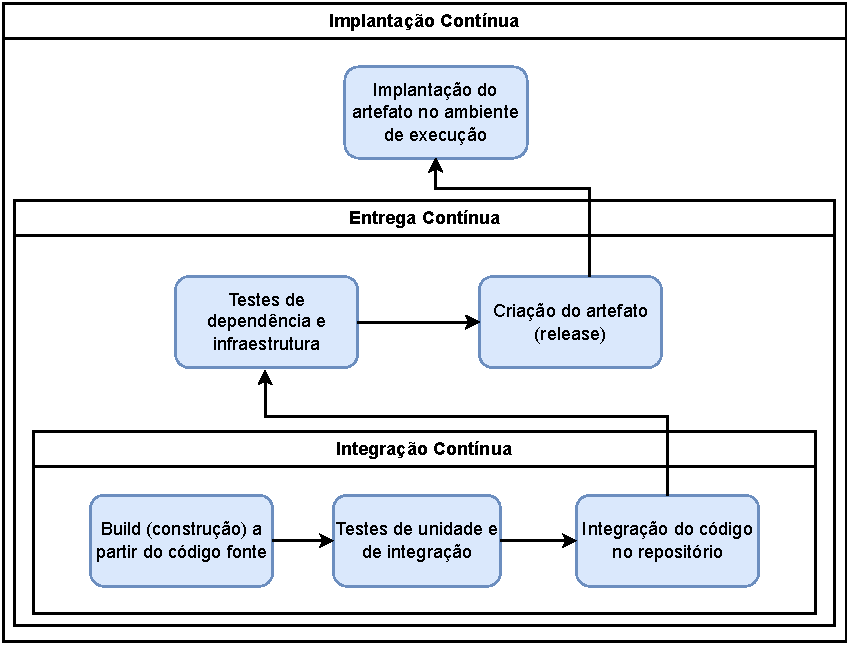
\includegraphics[scale=1]{Imagens/CICD.drawio.pdf}
	\end{center}
	\legend{Fonte: Autor}
\end{figure}
% With continuous delivery, the software is built so that it can be deployed to production at any time. Then you can trigger the deployments manually or move to continuous deployment where deployments are automated as well. \cite{gitlab-ci-cd}

% At Thoughtworks, we're big fans of continuous integration servers - indeed we led the original development of CruiseControl and CruiseControl.NET, the widely used open-source CI servers. Since then we've also built the commercial Cruise CI server. We use a CI server on nearly every project we do and have been very happy with the results. (MartinFowler)

% Continuous Delivery means you ensure every change can be deployed to production. Continuous Deployment means you deploy every change. - Martin fowler https://twitter.com/martinfowler/status/598918601190580224?lang=en

% CI/CD, continuous integration/continuous delivery, é um método para entregar aplicações com frequência aos clientes. Para isso, é aplicada a automação nas etapas do desenvolvimento de aplicações. Os principais conceitos atribuídos a esse método são a integração, entrega e implantação contínuas. Com o CI/CD, é possível solucionar os problemas que a integração de novos códigos pode causar para as equipes de operações e desenvolvimento (o famoso "inferno de integração"). Especificamente, o CI/CD aplica monitoramento e automação contínuos em todo o ciclo de vida das aplicações, incluindo as etapas de teste e integração, além da entrega e implantação. Juntas, essas práticas relacionadas são muitas vezes chamadas de "pipeline de CI/CD" e são compatíveis com o trabalho conjunto das equipes de operações e desenvolvimento com métodos ágeis. citar \url{https://www.redhat.com/pt-br/topics/devops/what-is-ci-cd}

% CI/CD falls under DevOps (the joining of development and operations) and combines the practices of continuous integration and continuous delivery. CI/CD automates much or all of the manual human intervention traditionally needed to get new code from a commit into production such as build, test, and deploy, as well as infrastructure provisioning. With a CI/CD pipeline, developers can make changes to code that are then automatically tested and pushed out for delivery and deployment. Get CI/CD right and downtime is minimized and code releases happen faster. citar \url{https://about.gitlab.com/topics/ci-cd/}

% As you traverse environments from non-prod to the staging environment and eventually to production, the number of endpoints you deploy to increases. Continuous Deployment focuses on the path of least resistance to get the software into the needed environment(s). citar \url{https://harness.io/blog/continuous-delivery-vs-continuous-deployment}

% Being strategic in where to apply parts of your test suite is needed in order to avoid overburdening the Continuous Integration process. A line in the sand should be that Continuous Integration tackles artifact-centric confidence-building (for example, unit tests and artifact scans). Tests that take into account other artifacts and dependencies and/or application infrastructure are better-suited for the Continuous Delivery process. After the build is checked into a central repository, the next step to getting your idea into production is the promotion/deployment process. citar \url{https://harness.io/blog/continuous-delivery-vs-continuous-deployment}

\subsection{Integração contínua (CI)}
CI (\emph{Continuous Integration} - Integração contínua) é uma prática no desenvolvimento de \emph{software} onde os desenvolvedores integram o código em um repositório compartilhado frequentemente. Muitos times afirmam que essa prática leva a uma grande redução nos problemas de integração e os permite desenvolver \emph{software} coeso mais rapidamente. Além disso, melhora a identificação do progresso do desenvolvimento, facilita a identificação e remoção de falhas e \emph{bugs}, e aumenta a experiência e a confiança do time nos testes e \emph{build} do código desenvolvido. A integração contínua por sí só requer apenas uma ferramenta de controle de versão para ser feita, mas existem práticas bem consolidadas na indústria do desenvolvimento de \emph{software} que incrementam esse processo, apresentadas a seguir. \cite{martin-fowler-continuous-integration}.

% como Git\footnote{Git: \url{https://git-scm.com/}})
% Aplicação dessa prática no projeto: PIPELINE NO GITHUB ACTIONS

\subsubsection{Uso de apenas um repositório fonte}
Deve haver apenas um repositório por projeto ou microsserviço, compartilhado por toda a equipe desenvolvedora e contendo tudo aquilo que é necessário para uma instalação rápida e funcional do ambiente de desenvolvimento. Isso inclui mas não é limitado a - código, \emph{scripts}, migrações e esquemas de bancos de dados, arquivos de propriedades e configurações de IDE. Além disso, o conteúdo do repositório deve estar disponível para todos, assim aumentando a visibilidade e facilitando o monitoramento do progresso do conteúdo \cite{gitlab-ci-cd,martin-fowler-continuous-integration}.

% Aplicação dessa prática no projeto: DOCKER e DOCKER-COMPOSE

\subsubsection{\emph{Build} rápido}
Um \emph{build} (construção) da aplicação trata-se da transformação dos arquivos no repositório em um programa iniciável. \emph{Builds} lentos afetam negativamente a integração contínua, atrasando integrações e diminuindo a frequência do \emph{feedback}. Além disso, todas as etapas do \emph{build} devem ser simples de executar, idealmente por meio de um único comando \cite{martin-fowler-continuous-integration}.


\subsubsection{Automação de testes em novas integrações}
As integrações de cada novo \emph{commit} no repositório devem ser testadas, o que pode ser uma tarefa árdua e demorada dependendo de como o \emph{build} da aplicação é feito e da quantidade de testes, especialmente se feitos manualmente. Desse modo, deve-se elaborar uma bateria de testes, e executá-la de forma automática a cada novo \emph{build}, para assim detectar falhas rapidamente e aumentar a qualidade do \emph{software} \cite{gitlab-ci-cd,martin-fowler-continuous-integration}.

% build: Instalação de dependências e assets, minificação, compilação, linkagem, 

\subsubsection{Servidor de integração}\label{subsecao-servidor-de-integracao}
Muitas vezes não é possível (nem recomendado) executar todos os passos do \emph{pipeline} de integração na máquina do desenvolvedor, seja por questões de tempo, de capacidade computacional ou pela falta de garantia de que o desenvolvedor realmente executará os passos. Nesses casos, recomenda-se providenciar um local que centralizará a integração do novo código desenvolvido com o repositório principal. Tal local é chamado de \emph{CI Daemon}, ou servidor de integração, e ele é responsável por executar todos os passos do \emph{pipeline} de integração, assim como disponibilizar informações e relatórios sobre os passos executados. Também é recomendado estabelecer condições para que a integração do novo código seja efetuada, tal como a execução bem-sucedida de todos os testes, assim garantindo que apenas o código que cumpra tais condições seja integrado e consequentemente aumentando a qualidade do código e do produto \cite{martin-fowler-continuous-integration,continuous-delivery-jez-humble}.

\subsubsection{Estabilidade do ramo principal}
Um dos principais motivos para se usar a integração contínua é a garantia de que a equipe sempre estará trabalhando a partir de uma base de código estável. Se o ramo principal está instável, é tarefa de toda a equipe resolver o problema o mais rápido possível, pois nenhum código poderá ser desenvolvido a partir daquele ramo até que esteja estável e confiável novamente. Geralmente o melhor meio de resolver esse problema é reverter os \emph{commits} problemáticos, mas se a solução for simples, integrar um novo \emph{commit} pode ser suficiente. \cite{martin-fowler-continuous-integration}.

% A continuous integration server acts as a monitor to the repository. Every time a commit against the repository finishes the server automatically checks out the sources onto the integration machine, initiates a build, and notifies the committer of the result of the build. The committer isn't done until she gets the notification - usually an email.

% Not everyone prefers to use a CI server. Jim Shore gave a well argued description of why he prefers the manual approach. I agree with him that CI is much more than just installing some software. All the practices here need to be in play to do Continuous Integration effectively. But equally many teams who do CI well find a CI server to be a helpful tool.

\subsection{Entrega/Implantação contínua (CD)}
CD significa entrega contínua e/ou implantação contínua, conceitos relacionados e às vezes usados alternadamente. Em ambos os casos, trata-se da automação de fases avançadas do \emph{pipeline} de implantação. A entrega contínua é uma evolução da integração contínua e envolve todo o ciclo do projeto, até a criação da nova versão da aplicação, mas a implantação dessa nova versão no ambiente de execução ainda é feita manualmente. A implantação contínua engloba a entrega contínua e adiciona o passo de automatizar a implantação da nova versão no ambiente de execução. A finalidade da entrega contínua é garantir o mínimo de esforço na implantação de novas alterações, enquanto a da implantação contínua é sempre manter o ambiente de execução atualizado com as últimas alterações. A adoção da implantação contínua deve ser ponderada, pois para alguns negócios é preferível uma taxa de implantações mais baixa. A arquitetura de microsserviços tem uma ótima afinidade com a implantação contínua, por ser naturalmente modularizada e mais facilmente testável \cite{gitlab-ci-cd,redhat-ci-cd}.

Os benefícios da entrega contínua incluem: risco reduzido na implantação, pois como as mudanças são menores, há menos possibilidades de problemas, e caso haja, o conserto é mais simples; visualização do progresso, que não será simplesmente por trabalho "completo", mas sim por trabalho entregue; e \emph{feedback} do usuário mais rápida e frequentemente \cite{martin-fowler-continuous-delivery}.

\subsubsection*{Anti-padrão em CD: gerenciamento manual de ambientes}
Diferenças entre ambientes que deveriam ser iguais, ou o mais similares possível, por exemplo homologação e produção. Diferenças entre réplicas. Resulta em implantações não confiáveis. Deve-se tratar a configuração de ambiente como código, com versionamento e automatizado. \cite{continuous-delivery-jez-humble}

\subsubsection*{Anti-padrão em CD: implantação manual}
Realizar os passos da implantação manualmente resulta em uma implantação lenta e propícia a erros. Recomenda-se automatizar a implantação o suficiente para que possa ser feita com apenas o clique de um botão, ou, caso seu negócio permita, ser completamente automática. \cite{continuous-delivery-jez-humble}

\subsubsection*{Anti-padrão em CD: baixa frequência de implantação}
Implantar o \emph{software} com baixa frequência resulta em pouca colaboração e entendimento entre a equipe de desenvolvimento e a de operações. Quanto mais frequente é a implantação, menor é a dificuldade dela. \cite{continuous-delivery-jez-humble, martin-fowler-frequency}

\subsubsection{Estratégias de lançamento}\label{estrategias-implantacao}
Estratégias de lançamento dizem respeito a como atualizar uma aplicação em produção, e a escolha da estratégia depende de fatores como risco, tempo de inatividade e a necessidade de controle sobre a liberação de funcionalidades. Algumas estratégias fazem uso de \emph{dark launching} (lançamento escuro), que significa que algumas funcionalidades estão disponíveis para alguns usuários sem que eles saibam, permitindo testes e monitoramento com usuários reais antes do lançamento completo. É importante notar que implantação (\emph{deploy}) e lançamento (\emph{release}) são conceitos distintos, embora frequentemente usados de forma intercambiável. Implantação refere-se à ação técnica de implantar a nova versão do \emph{software} em um ambiente de execução, enquanto lançamento é o momento em que a versão é disponibilizada aos usuários, uma decisão que envolve considerações de negócio.

Ao separar implantação e lançamento, as equipes técnicas podem realizar implantações mais ágeis, por não depender de decisões de negócios. Isso permite que a área técnica trabalhe com mais autonomia e frequência nas implantações, enquanto a área de negócios ainda pode decidir o melhor momento para liberar a nova versão para o público, alinhando o lançamento com objetivos estratégicos. A seguir são apresentadas algumas estratégias comuns de lançamento.

% Alguns fazem uso de padrões `dark launching`, onde alguns usuarios usam funcionalidades e outros não
% Deploy: Implantação, é uma decisão técnica
% Release: Lançamento (a implantação que o usuário usa). É uma decisão de negócio.
% Muitas vezes deploy e release são usados alternadamente com o mesmo significado
% Ao separar essas duas etapas, a equipe técnica pode trabalhar de forma mais ágil e independente, realizando os deploys conforme necessário. A área de negócios, por sua vez, pode decidir o melhor momento para liberar a nova versão para os usuários, de acordo com os interesses do negócio.

% Todo pipeline é relacionado com testes e o feedback deles. Um software que é difícil de testar, ou não possui testes, já não atende a integração contínua, menos ainda a entrega contínua.

% Deployability define a facilidade de implantar o software. Microsserviços, por exemplo, possuem vantagens aqui.

% Embora seja teoricamente possível realizar entrega contínua sem integração contínua, praticamente é inviável, pois entregar alterações que ainda não foram devidamente integradas no repositório não faz sentido do ponto de vista do desenvolvimento de \emph{software} em equipes 

% Algumas das principais abordagens incluem Blue-Green Deployment, Canary Deployment, Rolling Deployment e Feature Flags

\subsubsubsection*{\emph{Blue-Green Deployment}}
No \emph{Blue-Green Deployment}, quando deseja-se lançar uma nova versão, são mantidos um ambiente de produção com a versão antiga (\emph{Blue}) e um com a versão nova (\emph{Green}). Para permitir uma transição suave entre versões para os usuários, o tráfego é redirecionado para o ambiente novo após a validação da nova versão, favorecendo uma atualização segura e diminuindo riscos. Além disso, caso ocorra algum problema, é possível rapidamente reverter para o ambiente antigo, sendo necessário apenas mudar o redirecionamento.
\cite{martin-fowler-bluegreen}

\subsubsubsection*{\emph{Canary Release}}
No \emph{Canary Release}, a nova versão é disponibilizada para um número gradual dos usuários. Inicialmente, a nova versão é implantada em uma parte restrita do ambiente de execução, sem tráfego significativo, permitindo testes preliminares. Em seguida, um subconjunto de usuários é direcionado para essa versão, possibilitando a detecção de falhas ou problemas antes que a atualização afete todos os usuários. Se nenhum erro crítico for identificado, a distribuição da nova versão ocorre de forma progressiva, garantindo maior controle e diminuindo riscos. Essa abordagem permite um monitoramento mais eficiente do desempenho e da estabilidade da nova versão, também possibilitando uma fácil reversão (\emph{rollback}) da implantação caso necessário, assim protegendo a experiência dos usuários.
\cite{canary-release}

\subsubsubsection*{\emph{Feature Toggles}}
Com os \emph{Feature Toggles}, também conhecidos como \emph{Feature Flags}, funcionalidades podem ser ativadas ou desativadas sem a necessidade de modificar o código-fonte ou realizar novas implantações. Essa abordagem permite maior flexibilidade no lançamento de novas funcionalidades, facilitando testes A/B, lançamentos graduais e controle operacional de determinadas partes do sistema, inclusive podendo ser feitas de forma que o usuário decida se quer ou não usar a nova funcionalidade. Existem diferentes categorias de Feature Toggles, incluindo \emph{Release Toggles}, que gerenciam a ativação progressiva de novas features; \emph{Experiment Toggles}, que suportam testes controlados; \emph{Ops Toggles}, que ajustam o comportamento do sistema em tempo de execução; e \emph{Permissioning Toggles}, que regulam o acesso de usuários a funcionalidades específicas. No entanto, o uso excessivo desses \emph{toggles} pode aumentar a complexidade do código, tornando essencial a adoção de boas práticas para seu gerenciamento, como a documentação clara e a remoção de \emph{toggles} obsoletos.
% podendo até ser escolha do usuário se ele quer usar a nova versão ou a antiga. 
\cite{feature-toggles}

% Um deployment pipeline é um fluxo em que o artefato passa e cada etapa incrementa e agrega mais segurança ao se aproximar do ambiente de produção. Deploys de baixo risco são aqueles experimentais, contínuos, atualizações pontuais acompanhadas. Devemos separar a ideia de "deploy" e "publicação".Otimizar para resiliência é prevenir erros. No contexto de integração e entrega contínua temos o deploy contínuo. As equipes de desenvolvimento normalmente possuem divisões, como as pessoas do QA,deploy e operações. As tarefas são delegadas para os subgrupos durante o projeto. Equipes separadas que mal se comunicam dificultam o andamento do trabalho, aumentam a possibilidade de problemas e atrasam os deploys. A entrega contínua também exige uma mudança no comportamento e na cultura da empresa: as pessoas precisam trabalhar integradas.

% Continuous deployment enables organizations to automatically deploy their applications – eliminating the need for human intervention. With continuous deployment, DevOps teams set the criteria for code releases ahead of time and when those criteria are met and validated, the code is deployed into the production environment. Thanks to this type of automation, organizations are able to be more nimble and get new features into the hands of users faster. \cite{gitlab-ci-cd}

% While you can do continuous integration without continuous delivery or deployment, you can’t really do CD without already having CI in place. That’s because it would be extremely difficult to be able to deploy to production at any time if you aren’t practicing CI fundamentals like integrating code to a shared repo, automating testing and builds, and doing it all in small batches on a daily basis. \cite{gitlab-ci-cd}

% Where Continuous Deployment focuses on the actual deployment, Continuous Delivery focuses on the release and release strategy. An elusive goal would be a “push of a button” to get changes into production. That “push of a button” is Continuous Delivery. \cite{harness-ci-cd}

\section{DevOps}

Historicamente, existe uma diferença no foco do trabalho entre desenvolvedores e operadores que já está arraigada em muitas empresas que lidam com o desenvolvimento de \emph{software}. Enquanto por um lado as equipes de desenvolvimento tentam ser o mais eficientes possível, entregando tarefas completas sempre que possível, por outro, a equipe de operações valoriza a estabilidade, considerando cada alteração como uma possível causa de problemas. Assim, uma equipe preza pela velocidade em novas funcionalidades, enquanto a outra, pela estabilidade. Com isso em mente, integrantes da indústria do desenvolvimento de \emph{software} começaram a conceber um movimento, chamado DevOps, com o objetivo de alinhar o foco das equipes e favorecer o trabalho em conjunto para conseguir alcançar uma entrega contínua e ao mesmo tempo manter o \emph{software} funcional no ambiente de execução.

DevOps, ilustrado na \autoref{figura_devops}, é um movimento cultural que visa a integração e otimização do processo de aprendizagem e colaboração entre os integrantes de equipes relacionadas ao desenvolvimento de \emph{software}. Ao contrário do que alguns pensam, não se trata de um cargo ou de um conjunto de ferramentas, mas sim de uma visão organizacional de trabalho que tem o objetivo de automatizar o ciclo de desenvolvimento do \emph{software} de modo que seja veloz, seguro e integrado, com foco nas necessidades do usuário e \emph{feedback} rápido. Práticas de DevOps, como integração e entrega contínua, são fundamentais para o sucesso de aplicações com arquitetura de microsserviços pelos benefícios que agrega ao time e ao desenvolvimento e operação da aplicação \cite{gitlab-devops}.

\begin{figure}[htb]
	\caption{\label{figura_devops}Ciclo DevOps}
	\begin{center}
	    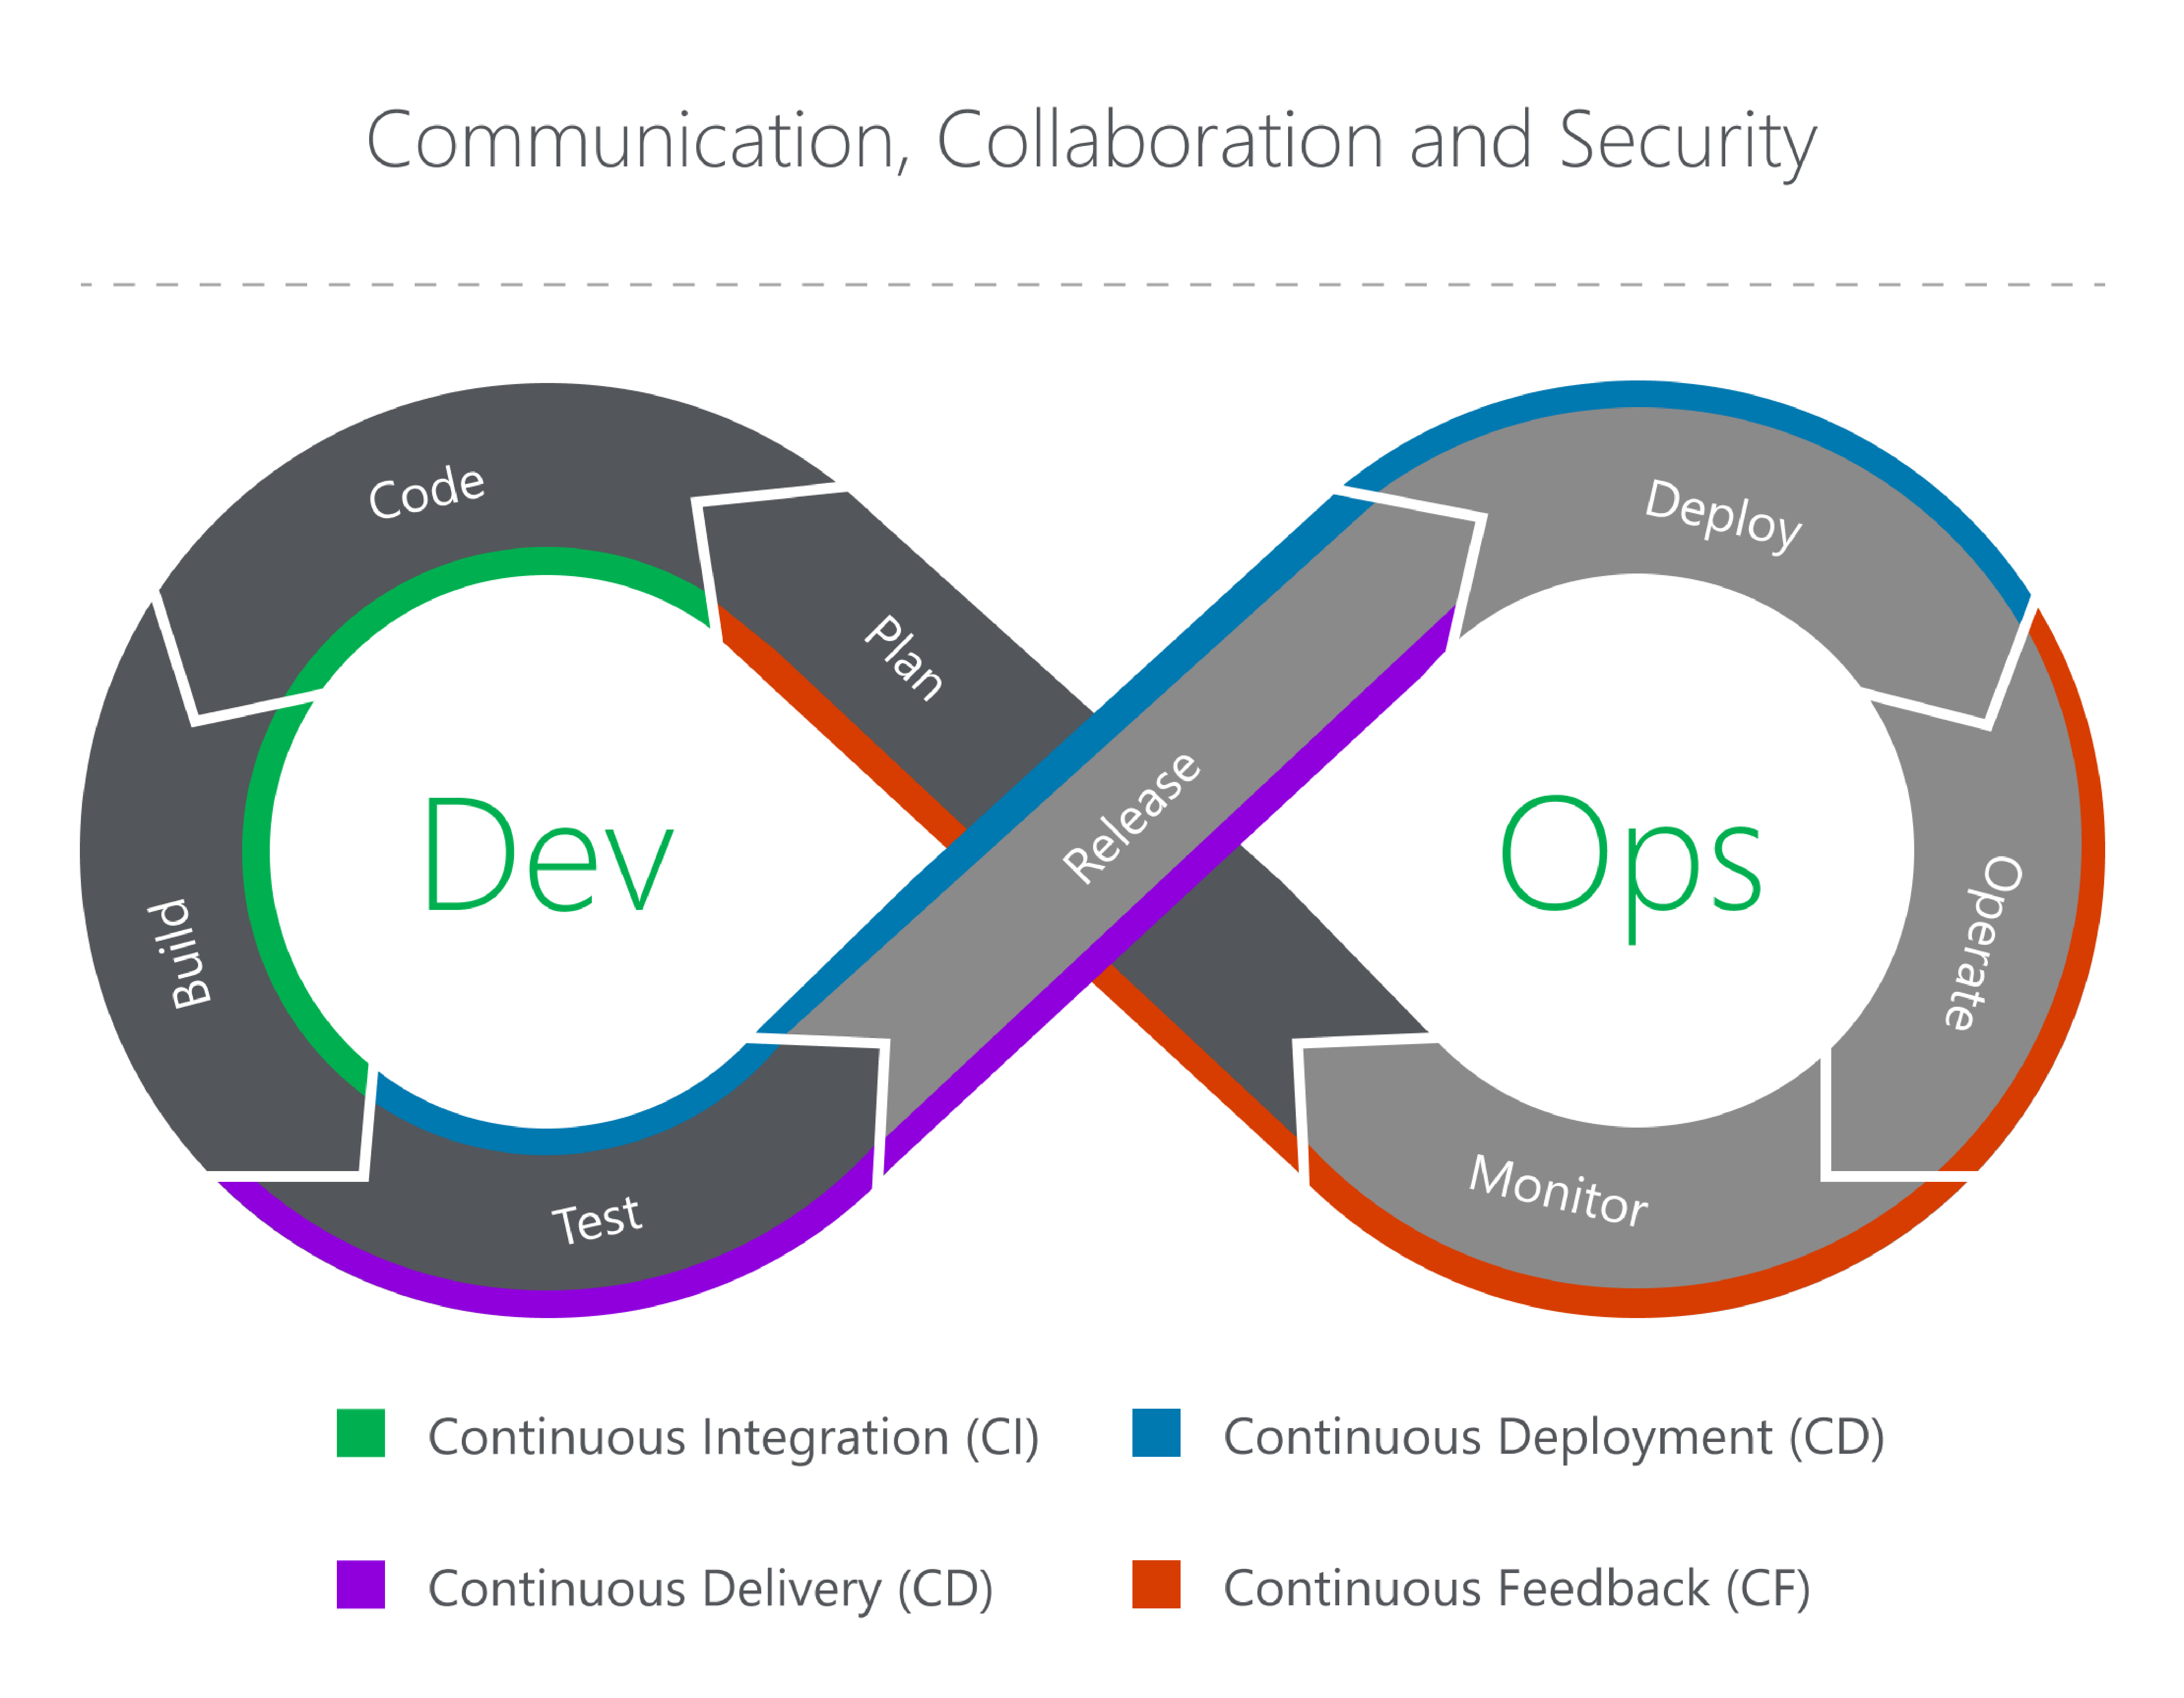
\includegraphics[scale=0.20]{Imagens/devops2.pdf}
	\end{center}
	\legend{Fonte: \citeonline{blog-devops}}
\end{figure}

% CI/CD is an essential part of DevOps and any modern software development practice. A purpose-built CI/CD platform can maximize development time by improving an organization’s productivity, increasing efficiency, and streamlining workflows through built-in automation, testing, and collaboration. As applications grow larger, the features of CI/CD can help decrease development complexity. Adopting other DevOps practices — like shifting left on security and creating tighter feedback loops — helps break down development silos, scale safely, and get the most out of CI/CD.

\section{Organização de código}
% Monorepo e polirepo são estratégias de organização de código.
% Para a organização de código no sistema de controle de versionamento, há duas abordagens - monorepo ou polirepo. Também tem a abordagem híbrida.

\subsection{Monorepo}\label{subsecao-monorepo}
Monorepo é uma estratégia de organização de código onde usa-se apenas um repositório no sistema de controle de versionamento para gerenciar múltiplos projetos. Ela é usada por diversas grandes empresas como Google, Facebook e Microsoft para gerenciar inúmeros projetos que formam um repositório enorme. O benefício mais tangível dessa abordagem é a simplificação do gerenciamento do versionamento dos projetos - como todos ficam em apenas um repositório, é mais fácil entender o histórico de mudanças e acompanhar o estado da aplicação, também facilitando restaurações de estados anteriores (\emph{rollbacks}). Segundo \citeonline{monorepo-polirepo-nicolas}, o uso dessa estratégia de organização de código também causa um impacto cultural nos times envolvidos com os projetos, encorajando código consistente e de alta qualidade e melhorando a cognição e o trabalho em equipe deles. Por outro lado, essa estratégia é uma violação do fator I da \hyperref[metodologia-12-fatores]{metodologia 12-fatores} e pode causar problemas, como pior desempenho da IDE e de ações como o \emph{build} devido ao grande tamanho do repositório; sobrecarga do servidor de integração devido ao maior número de operações no repositório; aumento do acoplamento entre os projetos caso os desenvolvedores não sigam práticas adequadas para manter o acoplamento baixo; e aumento na complexidade da automação de processos relacionados a integração, entrega e implantação contínua. \cite{monorepo-polirepo-semaphoreci, monorepo-do-or-do-not, monorepo-polirepo-nicolas}.

% Por que usar monorepo, que aumenta o acoplamento dos projetos, quando uma grande vantagem dos microsserviços é justamente o baixo acoplamento? 

% Simplifica a documentação . Um único \emph{pipeline} de implantação só que bem mais complexo. Testes de integração e de aceitação são mais fáceis de implementar. Usado por empresas grandes empresas como Google, Facebook e Uber.

% Pros
% 1. Since code for all the services lands in the same place, all issues related to multiple repositories — the proliferation of commits, PRs, code review, etc. disappear. Making the same change across multiple files like Kubernetes templates or logging settings becomes as easy as a global find & replace.
% 2. We also planned on developing a single CI/CD pipeline for all the services, to not have to monitor multiple jobs for failures. More on this below.
% 3. Also, the adoption of a monorepo would not compromise our microservice architecture, like decreasing the number of services would. Despite the move to a single repository each service would remain decoupled from others. All in all, the benefits sounded promising.

% many large enterprises benefit from a mono-repository for source code management because of the improved team cognition that results from eroding barriers between teams and from influencing enhanced teamwork quality.
% it has observed that the benefit of monorepo is the cultural impact. It has asserted that a monorepo facilitates cultural change and enables a holistic team cognition that ensures high quality work and improves communication, while preserving necessary autonomy.
% more research is necessary on source control repository structures and their direct impacts on team cognitions. \cite{monorepo-polirepo-nicolas} 
% a monorepo or polyrepo architecture involves a comparison of tradeoffs while still highlighting that monorepos "encourages consistent and high-quality code, and empowers engineers

\subsection{Multirepo}
Multirepo, ou polirepo, é uma estratégia de organização de código onde usa-se múltiplos repositórios no sistema de controle de versionamento para o gerenciamento de múltiplos projetos. Na arquitetura de microsserviços isso geralmente significa ter um repositório para cada microsserviço e é a estratégia mais comum de organização de código. Suas vantagens em contraste com o monorepo incluem: tamanho razoável do repositório; escopo do repositório bem definido; definição de permissões diferentes para cada projeto; e operações no repositório têm melhor desempenho. Essa abordagem é mais adequada quando não há necessidade de gerenciar cuidadosamente a versão da aplicação como um todo e esse versionamento é transparente para os usuários \cite{monorepo-polirepo-semaphoreci}.

% Usar um pipeline para cada repo implica em uma microimplantação. É mais cabível para aplicações praticando implantação contínua dos microsserviços, onde o gerenciamento da versão não tem grande importância. Requer mais esforço do que o monorepo mas oferece mais autonomia

% \subsection{Híbrido}

% O que é mais natural é utilizar um repositório para cada projeto, de um tamanho razoável com escopo bem definido. Essa forma de organização é chamada Multi-repo. Há possibilidade de definir permissões de acesso por projeto. clone, commit e build do projeto é mais simples e rápido

% No entanto, nos últimos anos, surgiu uma nova forma de organização dos nossos projetos dentro de repositórios. Empresas grandes de tecnologia como Google e Facebook não utilizam o esquema Multi-repo, porque são empresas que trabalham em inúmeros projetos de maneira concomitante. Empresas que atuam com outra dimensão de projetos utilizam o Mono-repo, ou seja, um único e gigantesco repositório que acumula todos os projetos.

% A desvantagem do segundo modelo é o repositório precisará ser realmente grande, e o build pode ser lento, talvez nem o Git seja mais a ferramenta adequada para fazer o controle de versões para esta situação. Contudo, como temos apenas um grande repositório temos uma administração relativamente mais simples, então a verificação de padrões é facilitada. A refatorações são globais, afinal estão todos dentro da mesma base. 

% \subsection{Estratégias de ramificação} <<

% \section{Externalização/parametrização de configurações}\label{secao-externalizacao-de-configuracoes}
% TODO:? Falar sobre externalização da configuração do ambiente. Traz mais portabilidade ao código. Fazer paralelo com o 12-factor app fator 3

\section{Implantação em contêineres}
% TODO:? Elaborar melhor sobre orquestração de containers.

Contêineres configuram isolamentos lógicos em uma máquina, sendo leves, altamente flexíveis e permitindo paradas, alterações e reinicios velozes. Depois de desenvolvido o microsserviço, é altamente recomendado que ele seja implantado em um contêiner, para assim favorecer sua padronização e \hyperref[sec:portabilidade]{portabilidade}, também evitando interferências imprevistas com outros microsserviços. \cite{oracle_microservices}.
% Por se tratar mais de uma questão tecnológica do que de prática, a implantação em containers é melhor discutida no capítulo 5
% Docker\footnote{Docker: \url{https://www.docker.com/}} 

% A container is a standardized unit of software, used to develop, ship and deploy applications. Containers are managed using a container engine, such as Docker. The container engine provides the tools that are necessary to bundle all the application dependencies as a container. You can use the Docker engine to create, deploy, and run your microservices applications in containers. Microservices running in Docker containers have the following characteristics:

% Standard: The microservices are portable. They can run anywhere.
% Lightweight: Docker shares the operating system (OS) kernel, doesn’t require an OS for each instance, and runs as a lightweight process.
% Secure: Each container runs as an isolated process. So the microservices are secure.

% The process of containerizing a microservice involves creating a Dockerfile, creating and building a container image that includes its dependencies and the environmental configuration, deploying the image to a Docker engine, and uploading the image to a container registry for storage and retrieval. \cite{oracle_microservices}

\section{Testes}
% Testes é um assunto complexo, especialmente em arquiteturas distribuidas.

Tradicionalmente, um \emph{build} engloba tudo que é necessário para que um programa possa executar. Entretanto, só porque um programa executa não significa que ele fará o que é esperado. Para tanto, deve-se testar o programa, idealmente de forma automática e para toda funcionalidade, assim falhas e \emph{bugs} podem ser descobertos antes de serem lançados. Existem inúmeros tipos e abordagens de testes de \emph{software}, porém é impossível ter uma cobertura completa de testes. Trata-se, portanto, de quão testada é a aplicação - quanto mais bem testada, pelo uso de abordagens diversas e apropriadas, maior é a confiabilidade e a qualidade do sistema. Entretanto, é importante também não só automatizar a bateria de testes, mas também prezar pelo seu desempenho, pois testes demorados tornam-se um obstáculo para a integração e \emph{feedback} contínuos, portanto antes de sair criando vários testes complexos para a aplicação, deve-se avaliar se a confiabilidade resultante justifica a complexidade de implementação e execução. \cite{martin-fowler-continuous-integration,livro-building-microservices}


Na arquitetura de microsserviços, o processo de testes torna-se mais abrangente, por haver mais pontos passíveis de falha, e mais complexo, por se tratar de um sistema altamente distribuido. Além disso, um microsserviço, de maneira isolada, também pode ser testado com tipos de testes comumente usados em aplicações monolíticas, como testes de unidade e de serviço.
% porém não existe uma definição formal de quais testes devem ser utilizados em quais casos, 
% Existem inúmeros tipos e abordagens de testes de \emph{software}, que compõem diversos livros por ótimos autores focados no assunto, que explicariam melhor do que eu jamais poderia, portanto este trabalho não entrará em detalhes sobre como implementá-los ou como funcionam, e serão apenas apontados algumas estratégias apropriadas de testes no contexto de aplicações com arquitetura de microsserviços.

% Recomenda-se usar todas as abordagens comuns de testes, como \emph{mocking}, testes de unidade, testes de regressão e testes funcionais. \cite{design-monitoring-testing-waseem}

\subsection{Testes de unidade}
Testes de unidade verificam funções ou métodos isoladamente, sem depender de serviços externos ou conexões de rede. Esse tipo de teste é voltado para desenvolvedores, ajudando-os a detectar \emph{bugs} e facilitando a refatoração do código, por garantir que alterações estruturais não quebrem funcionalidades existentes. Além disso, esses testes têm custo muito baixo, tanto para implentar quanto para executar, então é muito difícil uma aplicação chegar a um ponto que tenha testes de unidade demais. Em específico para linguagens interpretadas, eles podem ser acionados automaticamente ao modificar arquivos, proporcionando ciclos de \emph{feedback} mais rápidos \cite{livro-building-microservices}. 

\subsection{Testes de serviço}
Testes de serviço são projetados para testar microsserviços diretamente, ignorando interfaces de usuário. Em aplicações monolíticas, isso envolveria testar classes que fornecem serviços à essa interface, enquanto em sistemas baseados em microserviços, cada teste de serviço foca nas capacidades individuais de um microsserviço. Esses testes aumentam a confiança no comportamento do serviço, contanto que o escopo seja isolado, isso é, qualquer falha detectada deve estar restrita ao microsserviço testado. Para garantir esse isolamento, muitas vezes é necessário substituir todas as dependências externas por simulações delas (\emph{stubs}) \cite{livro-building-microservices}.

Alguns testes de serviço podem ser tão rápidos quanto testes unitários, mas a velocidade pode diminuir ao envolver bancos de dados reais ou conexões de rede com serviços simulados. Apesar de cobrirem um escopo maior que os testes unitários, tornando a identificação precisa de falhas mais difícil, eles ainda possuem menos variáveis do que testes de maior escala como os testes ponta a ponta, sendo assim mais confiáveis. \cite{livro-building-microservices}.

\subsection{Testes \emph{end-to-end} (ponta a ponta)}\label{subsecao-testes-endtoend}
Testes ponta a ponta verificam o fluxo completo de uma determinada funcionalidade da aplicação, incluindo integrações externas, assim envolvendo múltiplos microsserviços. \citeonline{livro-building-microservices} argumenta em seu livro “Building Microservices” que muitos desenvolvedores de microsserviços em escala dispensam testes ponta a ponta apesar do ótimo escopo que eles provêem, devido à grande quantidade de recursos que exigem para serem executados e por serem suscetíveis a problemas que não necessariamente tem relação com a funcionalidade testada, o que pode introduzir indeterminismo nos testes. É recomendado então usar testes ponta a ponta apenas quando o sistema não é muito grande, e a confiabilidade agregada por eles supera o custo de os manter. Conforme uma aplicação de microsserviços cresce, muitos desenvolvedores preferem aumentar a confiabilidade pelo uso de \hyperref[observabilidade-monitoramento]{monitoramento} avançado, \hyperref[estrategias-implantacao]{estratégias de implantação cuidadosas} e uso de \hyperref[subsecao-contratos-de-dados]{contratos de dados} orientados ao consumidor (CDCs) 
% que trata-se de especificar uma API com base em contratos compartilhados que ditam o que consumidor espera, facilitando testes de integração 
\cite{livro-building-microservices}.

% Dito isso, testes ponta a ponta ainda são muito comumente usados em aplicações com arquitetura de microsserviços. Cabe ao desenvolvedor estudar o contexto atual da aplicação para determinar se testes ponta a ponta são apropriados. \cite{design-monitoring-testing-waseem}

\subsection{Testes, testes e mais testes}
Além de recomendar os tipos de testes comuns em monólitos, \citeonline{Familiar2015} recomenda também testar os microsserviços conforme passam pelo \emph{pipeline} de implantação, incluindo: \textbf{Testes internos}, que testam as funções internas do serviço, incluindo uso de acesso de dados, caching e relacionados; \textbf{Testes de serviço}, que testam serviços da API e seus modelos associados; \textbf{Testes de protocolo}, que testam o serviço a nível de protocolo, chamando a API usando o protocolo escolhido; \textbf{Testes de composição}, que testam o serviço em cooperação com outros serviços no contexto de uma solução; \textbf{Testes de escalabilidade e taxa de transferência}, que testam a escalabilidade e elasticidade do microsserviço implantado; \textbf{Testes de tolerância a falha}, que testam a capacidade do microsserviço de se recuperar após uma falha; e \textbf{Testes de penetração}, que consiste em envolver uma empresa terceirizada de segurança de \emph{software} para realizar testes de penetração no sistema. \cite{Familiar2015}

% Testes fazem parte da construção do software. Devem ser realizados antes do commit. TDD pode ajudar neste processo. Deve-se prezar por um bom desempenho em testes, pois testes demorados podem ser uma barreira para a integração contínua. Testes automatizados são essenciais para a integração contínua.

% We identified 12 testing strategies (see Table 28), which are listed in our survey question, from the literature (e.g., [9, 6, 61, 63, 64, 65, 66, 67]).

\section{Comunicação}\label{secao-comunicacao}

% TODO:? Elaborar sobre o FastCGI. (geralmente usado para servidores de aplicação de linguagem interpretada como uma alternativa ao http)

No desenvolvimento de estruturas de comunicação entre diferentes processos, nota-se muitos produtos e abordagens que enfatizam o emprego de grande inteligência no próprio mecanismo de comunicação. Um exemplo disso é o Enterprise Service Bus (ESB), onde os mecanismos dessa abordagem geralmente incluem recursos sofisticados para roteamento, tratamento e transformação de mensagens e aplicação das regras de negócios \cite{martin-fowler-microservices}.

A comunidade de microsserviços favorece uma abordagem alternativa - \emph{endpoints} inteligentes e canais simples. Os microsserviços visam ser o mais desacoplados e coesos possível - eles possuem sua própria lógica de domínio e agem mais como filtros - recebendo uma solicitação, aplicando a lógica conforme apropriado e produzindo uma resposta. Isso geralmente é feito usando protocolos REST simples em vez de protocolos complexos como \emph{Web Service Choreography} ou orquestração por uma ferramenta central \cite{martin-fowler-microservices}.

O uso de APIs em conjunto com requisições HTTP é o método mais usado para realizar comunicação síncrona na arquitetura de microsserviços. Uma requisição HTTP é feita por um cliente (ou consumidor) para um dado provedor em um endereço, com o propósito de acessar um recurso dele. Por usar o \emph{Transmition Control Protocol} (TCP), é um método de comunicação confiável, mas não tão eficiente quanto poderia ser \cite{martin-fowler-microservices}.

Para comunicação assíncrona, sistemas de mensagens são amplamente usados. Quando um serviço precisa enviar informações a outro de modo assíncrono, ele envia uma mensagem para uma fila de mensagens e ela será armazenada até ser processada ou excluída. As filas de mensagens podem ser usadas para dividir um processamento pesado, para armazenar trabalho em \emph{buffers} ou lotes, ou para amenizar picos de cargas de trabalho \cite{amazon-filas-de-mensagens}.
% Cada mensagem é processada uma única vez, por um único consumidor. (?)

Embora menos comum, chamada de procedimento remoto (RPC) também é utilizado para realizar comunicação síncrona ou assíncrona nos microsserviços. Uma chamada de procedimento remoto se dá quando um programa faz com que um procedimento ou uma sub-rotina execute em um espaço de endereço diferente, comumente em outra máquina numa rede compartilhada. Essa chamada é feita como se fosse um procedimento local, isso é, o programador não precisa explicitar que se trata de um procedimento remoto. \cite{microsoft-grpc}.

De acordo com \citeonline{design-monitoring-testing-waseem}, \emph{API Gateway} e \emph{Backend for frontend} são os padrões de projeto mais utilizados na implementação da comunicação entre microsserviços. Eles são padrões similares - a diferença é que no \emph{Backend for Frontend} há um \emph{gateway} para cada tipo de cliente ou serviço de ponta.

% \subsection{Descoberta de serviços (\emph{Service Discovery})}
% TODO:? Elaborar sobre descoberta de serviços
% https://www.baeldung.com/cs/service-discovery-microservices
% https://medium.com/@jeslurrahman/understanding-service-discovery-in-microservices-architecture-2098b10e7439
% A descoberta de serviço é uma parte muito importante da comunicação entre microsserviços \cite{livro-building-microservices, service-discovery-baeldung}.

% Considerando que APIs são um tópico essencial na comunicação entre microsserviços, elas serão abordadas em maior profundidade na \autoref{boas-praticas-apis}.

\section{APIs}\label{boas-praticas-apis}

Considerando que APIs são uma parte crucial no desenvolvimento de microserviços, sendo responsável por grande parte da comunicação que se faz necessária para conectar tantos serviços separados e manter um funcionamento eficiente e livre de falhas, este trabalho apresentará diversas práticas no desenvolvimento de APIs.

\subsection{Contratos de dados}\label{subsecao-contratos-de-dados}
Contratos de dados representam os acordos formais sobre a estrutura e formato das informações trocadas entre uma API e seus consumidores, bem como definem os campos, tipos de dados e regras de comunicação usadas, garantindo uma interação sem inconsistências. Esses contratos também implicam num compromisso de manter o serviço correspondente funcionando e inalterado. Entretanto, com a evolução de um serviço, surge a necessidade de serem introduzidas melhorias e mudanças que podem impactar nesses contratos \cite{martin-fowler-microservices}.

Embora o versionamento de APIs seja uma solução tradicional para lidar com essa evolução, no contexto de microsserviços ele deve ser a última alternativa, pois tende a aumentar a complexidade da manutenção deles. Em vez disso, é recomendável projetar contratos que sejam flexíveis e resilientes a mudanças e introduzir apenas modificações aditivas nos provedores, assim não comprometendo consumidores existentes \cite{martin-fowler-microservices}.

Contratos de dados orientados ao consumidor (CDC) é uma abordagem para garantir que contratos de comunicação entre serviços estejam alinhados com as necessidades dos consumidores. Em vez de o provedor da API definir unilateralmente o contrato, os consumidores especificam suas expectativas, criando um contrato que o provedor formaliza por meio de testes automatizados a nível de serviço, permitindo que provedores validem continuamente se suas mudanças mantêm a compatibilidade com os consumidores sem aumentar a carga de testes consideravelmente, o que também reduz a necessidade de testes ponta a ponta, que tendem a ser custosos, como discutido na \autoref{subsecao-testes-endtoend} \cite{consumer-driven-contracts,livro-building-microservices}.

Ao projetar serviços de forma mais tolerante a mudanças e validar contratos dinamicamente, as equipes podem trabalhar de forma independente e lançar atualizações sem impactar outros sistemas. No entanto, para que essa abordagem funcione bem, é necessário uma boa colaboração entre as equipes e o uso de ferramentas adequadas que facilitem a criação e verificação automática desses contratos. Quando bem aplicado, o CDC promove maior estabilidade em sistemas distribuídos, permitindo que microsserviços evoluam de forma mais previsível e segura. \cite{consumer-driven-contracts}

\subsection{Formatos de dados}\label{subsecao-trocas-de-dados}
% TODO:? Essa parte deveria estar no capitulo de ferramentas..?
Atualmente JSON é um dos formatos mais populares para troca de dados na web, por ser facilmente lido tanto por humanos quanto por máquinas e não precisar de muitos metadados, como no formato XML. Em APIs, JSON é usado para enviar e receber requisições por meio do protocolo HTTP, sendo uma solução robusta para a comunicação entre cliente e servidor. Embora seja derivado do JavaScript, JSON também é suportado por muitas outras linguagens, seja nativamente ou por meio de bibliotecas. \cite{json_bourhis_2020}

Outra opção para trocas de dados é usar \emph{Buffers} de protocolo, ou \emph{Protocol buffers}, uma ferramenta de código aberto desenvolvida pelo Google que oferece um método de serialização de dados estruturados para envio de informações. Ela é neutra em linguagem e plataforma, é extensível e funciona como alternativa ao JSON na troca de dados. Essa ferramenta serializa os dados a serem enviados de modo a tornar o pacote mais leve e mais rápido, mas introduz uma complexidade extra. Por introduzir essa complexidade na troca de dados e não ser otimizada para quantidades de dados que excedem alguns megabytes, essa ferramenta não é recomendada para todo caso de uso \cite{google-protocol-buffers}.

\subsection{Códigos de status de respostas HTTP}
Esses códigos são números entre 100 e 599 que devem ser enviados com a resposta à requisição, cada um tendo um significado diferente, e cada centena sendo classificada em tipos diferentes de resposta. 100-199 representam respostas de informação, 200-299, respostas de sucesso, 300-399, tipos de redirecionamentos, 400-499, erros por parte do cliente e 500-599, erros por parte do servidor. Esse é um padrão definido na seção 10 da RFC 2616, e facilita o entendimento do cliente sobre o que aconteceu com a requisição à API. \cite{rfc_http_nielsen_1999, api-design-restfulapi}


% Dessa forma, serviços podem evoluir continuamente sem uso de versionamento, reduzindo o acoplamento entre serviços, simplificando a implantação e mantendo a flexibilidade da arquitetura.

% Para que essa evolução não resulte numa quebra do contrato de dados, deve-se projetar contratos que sejam flexíveis e resilientes a mudanças pode ser feito um versionamento da API e mantida a transparência com os consumidores, pela atualização da documentação, mas como mencionado na \autoref{secao-componentizacao}, essa prática não é recomendada \cite{martin-fowler-microservices}.

% Quando isso é feito, a versão da API muda de 2.3.7 para 2.4.0 ou para 2.3.8 dependendo do tamanho da mudança. Quando é necessário realizar alterações que descumprem o contrato, deve-se alterar a versão maior da API, por exemplo passando de 2.3.7 para 3.0.0. Nesses casos, é importante manter a versão anterior funcionando e inalterada, criando uma nova rota para acessar a versão nova, para que clientes usando a versão anterior não apresentem falhas.


% Para fazer o versionamento, pode-se usar o processo de versionamento de \emph{software} para representar os estados da API. Nesta técnica, usa-se três números para representar a versão, por exemplo "2.3.7". O primeiro representa a versão maior, o segundo, a versão menor, e o terceiro, o patch (pequena atualização para consertar ou melhorar algo) \cite{wiki_software_versioning_2022}.
% citar o curso da alura

\subsection{API Gateway}\label{boas-praticas-api-gateway}
% TODO:? Mudar o nome para Gateway, mover para uma seção, e tornar o texto mais genérico em vez de focado nas APIs.
% sessão Central Aggregating Gateway no livro building microservices
Na arquitetura de microsserviços, muitas vezes a comunicação acontece de muitos pra muitos, podendo um microsserviço enviar e receber requisições para e de múltiplos outros microsserviços. Caso essa comunicação não seja gerenciada de forma adequada, a escalabilidade e segurança do sistema podem ser afetadas negativamente. Conforme mais microsserviços são criados e os já existentes evoluem, torna-se inviável gerenciar tantos \emph{endpoints} em todo microsserviço que precisar usá-los. Uma solução para isso é usar um \emph{API Gateway}. \cite{livro-building-microservices}

Um \emph{API Gateway} é um padrão de projeto onde tem-se um servidor que age como uma porta única de entrada para as APIs de um sistema, padronizando e controlando o acesso a elas. Esse \emph{gateway} fica situado entre o consumidor e os microsserviços, e é responsável por redirecionar as requisições recebidas para os microsserviços apropriados, assim o gerenciamento das chamadas pode ser feita em apenas um lugar em vez de em cada consumidor. Além disso, nele também podem ser implementadas camadas de segurança, como autenticação, e de monitoramento, como \hyperref[subsecao-registros]{\emph{logging}}.

Outra vantagem é que esse \emph{API Gateway} pode agregar requisições, permitindo que o consumidor envie apenas uma requisição para o \emph{API Gateway} para recuperar informações de diferentes microsserviços, o que normalmente exigiria múltiplas requisições. Nesse caso, quando recebida a requisição do consumidor, o \emph{API Gateway} fica responsável por disparar as requisições correspondentes, agregar as respostas e as devolver ao consumidor.

Entretando, também há desvantagens no uso desse padrão: (1) cria-se um alto acoplamento entre os microsserviços e o \emph{API Gateway}, (2) ele pode se tornar um ponto massivo de falha e (3) se não escalado adequadamente, esse \emph{API Gateway} pode diminuir o de todas as requisições que passarem por ele \cite{microsoft-api-gateway}.

\subsection{Segurança em APIs}

\subsubsection*{Autenticação e autorização}

Incluir autenticação em uma API consiste em exigir uma prova de autorização do uso daquele recurso. A autenticação nas APIs é altamente recomendada por aumentar a segurança de forma simples, e existem várias formas de implementá-la, sendo um dos mais comuns pelo uso de \emph{JSON Web Tokens (JWT)}, definidos na RFC 7519 \cite{rfc_http_nielsen_1999}.

\subsubsection*{Validação de entradas}

Validar entradas significa verificar as requisições que chegam com o intuito de garantir que elas não contém dados impróprios, tais como injeções de SQL ou \emph{scripting} (execução de uma determinada sequência de comandos) entre sites. Essa validação deve ser implementada tanto em nível sintático como em semântico, isso é, tanto impondo correção da sintaxe quanto impondo correção de valores \cite{api-design-restfulapi}.

\subsubsection*{Certificado Secute Socket Layer (SSL)}
Usar um certificado SSL permite que o protocolo HTTPS seja usado em vez do HTTP, criptografando as informações que estão trafegando, aumentando a privacidade da informação trafegada. \cite{api-design-restfulapi}

\subsubsection*{Limitação de taxa de requisições}
Limitar a taxa de requisições é um jeito de proteger a infraestrutura do servidor nos casos de acontecerem grandes fluxos de requisições, tal como em um ataque de \emph{DoS} (negação de serviço). Clientes terão seu acesso bloqueado caso enviem uma quantidade de requisições acima do limite determinado \cite{api-design-restfulapi}.

% \subsubsection*{Compartilhar o mínimo possível}
% Compartilhar o mínimo possível é uma medida de segurança genérica que pode ser adotada em qualquer microsserviço. Especificamente nas APIs, é recomendado retornar apenas os dados necessários para o cliente. Muitas ferramentas usadas para implementar APIs incluem por padrão informações como se fossem marcas d'água, mas que podem ser removidas, tal como headers "X-Powered-By", que vazam informações do servidor que podem auxiliar usuários mal-intencionados \cite{rapidAPI-twitter}.

% \subsection{Testes isolados}
% Testar uma API isoladamente serve para determinar se ela atende a parâmetros pré-definidos ou não. Tais parâmetros podem ser o cumprimento da funcionalidade, a confiabilidade, a latência, o desempenho, e a segurança. Quando um teste de API falha, deverá ser possível saber precisamente onde o problema se encontra, assim aumentando a velocidade de desenvolvimento e a qualidade do produto.

% Why should you perform API testing?
% - Testing your APIs timely helps to ensure your app is up all the time.
% - It helps to detect API security and performance issues.
% Benefits of API Testing
% - When API tests fail, you will know precisely where the issue lies that crashed the system.
% - As data is exchanged via XML or JSON, you can write API tests in your preferred language.
% - API testing also helps to release the next API version faster. \cite{rapidAPI-twitter}

\subsection{\emph{Caching}}
Às vezes referido como \emph{cachear}, salvar informações em \emph{cache} pode melhorar significativemente o tempo de busca da informação pelo cliente. Em uma API podem haver múltiplas requisições para a mesma informação em um curto intervalo de tempo, e para cada requisição será necessário buscar a informação. Entretanto, se a informação estiver salva no \emph{cache}, não será necessário buscar essa informação, o que melhora o tempo de resposta da API, especialmente em \emph{endpoints} que frequentemente retornam a mesma resposta \cite{api-design-restfulapi}.

\subsection{Comprimir os dados}
A transferência de cargas grandes pode diminuir a velocidade da API. Comprimir os dados auxilia nesse problema, diminuindo o tamanho da carga e aumentando a velocidade de transferência. Uma possibilidade é usar \hyperref[subsecao-trocas-de-dados]{\emph{buffers} de protocolo} \cite{api-design-restfulapi}.

\subsection{Documentação}
Uma API é apenas tão boa quanto sua documentação, e a falta de informações claras sobre seu uso pode ser um motivo suficiente para não utilizá-la. A documentação deve ser bem formatada e de fácil navegação, preferencialmente usando ferramentas populares para reduzir a curva de aprendizado dos desenvolvedores. Além disso, é importante incluir exemplos práticos de requisições e respostas, permitindo que os usuários testem facilmente a API. \cite{api-design-restfulapi}

% There are various compression methods available, a common one being GZIP. \cite{rapidAPI-twitter}

% \subsection{Evitar trazer ou buscar resultados a mais ou a menos}
% Over-fetching results in unnecessary and unusable data, and under-fetching results in an incomplete response. Good architecture, planning, and appropriate API management tools are essential to avoid these. \cite{rapidAPI-twitter}

\subsection{Paginar e filtrar}
Em APIs, a paginação separa e categoriza resultados, enquanto a filtragem garante que apenas os resultados relevantes de acordo com os parâmetros da requisição são retornados. A paginação e a filtragem de resultados reduzem a complexidade da resposta e a quantidade de dados trafegados, assim poupando recursos \cite{api-design-restfulapi}.

% \subsection{PATCH ou PUT}
% Quando é necessário modificar um recurso em uma API, usa-se os métodos HTTP PUT ou PATCH. Enquanto PUT atualiza o recurso inteiro, PATCH atualiza apenas uma parte específica do recurso, assim usando uma carga de dados menor. Portanto, quando possível deve-se usar PATCH em vez de PUT para modificar um recurso \cite{rapidAPI-twitter}.

\section{Observabilidade e Monitoramento}\label{observabilidade-monitoramento}
% Ambos são uma parte muito importante do \emph{Site Reability Engineering} (SRE)
A observabilidade se trata de permitir a observação do estado de um sistema por meio da externalização de seu comportamento, e possui 3 pilares - \textbf{registros, métricas e rastreamento}. O monitoramento engloba a observabilidade e se trata de acompanhar o estado de um sistema por meio de registros e ações que podem ser tomadas como resposta a eles. O monitoramento é fundamental para promover o funcionamento adequado de um sistema, especialmente os com arquiteturas distribuidas, como a de microsserviços. Com essas arquiteturas, o monitoramento se torna ainda mais importante e complexo, entretanto, traz diversos benefícios, como redução de tempo médio de detecção e reparo de incidentes e favorecimento do cumprimento do Acordo de Nível de Serviço (\emph{Service Level Agreement} - SLA). Além disso, para que se possa ter um alto nível de automação, também é necessário haver um alto nível de monitoramento. As formas mais comuns de implementar monitoramento é por meio de \emph{logs} (registros) e métricas.

\citeonline{livro-sre-google} afirma que os aspectos mais importantes para se monitorar em sistemas distribuidos são latência (tempo de resposta do sistema), tráfego (demanda colocada no sistema), saturação (uso excedente de recursos do sistema) e erros occorridos, sejam erros explicítos (p. ex. erros 500 em uma requisição HTTP), implícitos (p. ex. respostas incorretas à requisição) ou por política (p. ex. tempo de resposta inadequado). O monitoramento desses aspectos muitas vezes são divididos em duas metodologias - RED e USE, que significam \emph{Rate, Errors, Duration} (Taxa, Erros, Duração) e \emph{Utilization, Saturation, Errors} (Utilização, Saturação, Erros), respectivamente. Enquanto RED foca na experiência do usuário, USE foca no funcionamento apropriado da infraestrutura, mas ambos são metodologias abrangentes e complementam um ao outro. \cite{livro-sre-google, grafana-blog}

% resource usage and load balancing as monitoring metrics, log management and exception tracking as monitoring practices are widely used \cite{design-monitoring-testing-waseem}

\subsection{\emph{Logs} (registros)}\label{subsecao-registros}

Um registro, ou \emph{log}, descreve o que aconteceu em um dado momento em um dado processo, provendo informações rastreáveis sobre o estado e a saúde dele. Manter um histórico de registros de uma aplicação é uma forma simples e eficiente de se implementar monitoramento, e é fortemente indicado para qualquer sistema, especialmente os distribuidos. 

Para favorecer uma eficiente escrita, leitura e operação dos registros, eles devem possuir ao menos: um código do evento ocorrido, uma mensagem descritiva, a condição tratada em caso de exceção ou erro e o período de retenção. Também deve-se padronizar o formato dos registros emitidos por todos os microsserviços e diferenciar entradas de erros, de avisos e de informação. Além disso, os registros devem ser agregados e organizados em um único lugar externo aos ambientes de execução da aplicação, para que possam ser facilmente consultados e para evitar perdas de informações, que podem acontecer especialmente em aplicações implantadas em contêineres e com escalamento horizontal. \cite{livro-sre-google-workbook}

% Um motivo importante para organizar os logs é rastrear as chamadas de uma execução. Devemos poder reconstruir uma operação a partir de um identificador. Isso é o equivalente à stack-trace de um sistema monolítico.

% Usar ferramentas de gerenciamento (APMs - Application performance management) para visualizar essas stack-traces.

\subsection{Métricas}
Uma métrica é uma medição de uma propriedade do sistema numa dada janela de tempo, e possui um objetivo específico, seja para questões de desenvolvimento, de infraestrutura ou mesmo de negócios e \emph{business inteligence}. Disponibilizar a porcentagem de uso de CPU em uma máquina, por exemplo, tem o objetivo de informar o operador sobre esse uso para que ele possa decidir que ações precisam ser tomadas. Recomenda-se ter métricas para todo ponto de atenção do sistema, que, é claro, variam de acordo com o sistema e suas regras de negócio, porém geralmente incluem uso de recursos, tempo de resposta e quantidade de acessos.

Enquanto registros precisam ser desenvolvidos, métricas apenas precisam de instrumentação pois muitas ferramentas já possuem as próprias métricas ou já existem métodos consolidados para as obter. Nos servidores web mais populares, por exemplo, as informações básicas sobre uma requisição já são gravadas por padrão.

É recomendado usar paineis de controle de alto nível para melhorar a visualização e monitoramento do status da aplicação e diversas outras informações operacionais e de negócio a partir de suas métricas \cite{martin-fowler-microservices}.

\subsection{\emph{Tracing} (rastreamento)}
Em aplicações com arquitetura distribuida, como os microsserviços, uma única requisição de um usuário irá frequentemente interagir com múltiplos serviços antes de retornar uma resposta, assim havendo possibilidade de ocorrer problemas em múltiplos locais diferentes. Rastreamento trata-se de acompanhar um fluxo transacional (geralmente iniciado por uma requisição de um usuário), desde onde foi originado até onde terminou, atribuindo um identificador único a cada fluxo, que será propagado em cada serviço por onde o fluxo passar. Isso provê visibilidade ponta a ponta sobre os fluxos no sistema, permitindo que desenvolvedores e operadores identifiquem problemas mais precisa e rapidamente, independentemente de onde eles ocorram. 
% PATTERN - DISTRIBUTED TRACING: https://microservices.io/patterns/observability/distributed-tracing.html

% \section{Agregando serviços (process agregator pattern)}
% Um padrão popular Agregar serviços de negócio em um único serviço mantém as funções em um nível mais alto. 

% Agrega serviços de negócio (É ainda mais alto nível)

% Fazem as chamadas para os serviços necessários e montam uma resposta adequada

% Deve ter uma lógica de processamento, e não ser apenas um proxy. No mínimo deve unir a resposta de diversos serviços

% Para construir um agregador, define-se um novo modelo para o sistema, que representará os dados agregados como um subnegócio

% A partir deste modelo, pensar na API que fornecerá as operações

% A ideia é relativamente simples, mas a implementação pode ser complexa

% \section{Pontos de entrada para cada tipo de cliente} 
% Gateway específico para determinados clientes

% Foco nas necessidades reais de determinados clientes

% Esses clientes podem ser clientes da API, como clientes HTTP, ou clientes de negócio mesmo

% Por exemplo, em vez de modificar a lógica de negócios, cria-se um novo 'edge', que receberá a resposta e modificará de acordo com a necessidade do cliente

% Uma possibilidade seria trabalhar apenas com edge services, e nenhum API gateway, isso é, não existiria um ponto único de entrada universal, mas sim um para cada tipo de cliente

% Para construir uma edge (ponta), deve-se primeiro Identificar o cliente e suas necessidades, e Construir contratos específicos para o cliente, isso é, ter recursos diferentes para cada cliente. Por exemplo, a URL pode ser diferente de cliente web para clientes mobile.

% \section{Do monólito aos microserviços}

% Separando serviços monolíticos

% - Separando serviços de domínio (Data Service):
%     . Usar Domain-Driven Design (DDD)
%     . Começar modelando o domínio, não pensando na persistância. Definir previamente as regras e o domínio (Programação orientada a interfaces), para então...
%     . Avaliar **quais ações serão disponibilizadas neste serviço**. (Ex: Inserir, editar, recuperar, exibir, etc...)
%     . Construir o serviço, pensando primeiro no contrato
%     . REST e RPC podem andar juntos

% - Separando serviços de negócio (Business Service):
%     . Identificar o processo que deve ser exposto
%     . Identificar os domínios que serão necessários nesse serviço
%     . Defina a API que será utilizada, focando no domínio e não nos dados. (Ex: Passar uma matrícula, e não um ID)
%     . Consumir serviços de domínio para executar os processos

% - Padrões
%     . Strangler pattern
%         ~ Quebrar um monolito, tirando as funcionalidades dele aos poucos
%         ~ Pode-se começar isolando os dados
%         ~ Ou pode-se começar isolando o domínio

%     . Sidecar pattern
%         ~ Compartilhar código sem que seja necessário criar um novo microserviço.
%         ~ Usa-se pacotes a parte, que podem ser facilmente instalados.
%         ~ Esses pacotes só precisam ser alterados em um lugar para ter efeito em todos os microserviços.
%         ~ Ex: pacotes do npm, do composer, do maven, etc

% \subsection{Identificação com DDD}\label{praticas-identificacao-com-ddd}

% a combination of domain-driven design and business capability is the most used strategy to decompose an application into microservices \cite{design-monitoring-testing-waseem}

% Um caminho possível para facilitar a identificação com DDD dos microsserviços seria em vez de projetar os modelos e os contextos limitados (conceito do DDD usado para limitar um domínio, dividindo modelos grandes e explicitando as relações entre eles) separando-os em camadas, deve-se juntar os contextos limitados com seus respectivos modelos, e procurar por possíveis pontos de separação da aplicação - um lugar onde a linguagem muda, por exemplo. Isso resultaria em um ponto de partida para separar as partes e formar uma arquitetura de microsserviços. \cite{Familiar2015}

% If you are currently working with a complex layered architecture and have a reasonable domain model defined, the domain model will provide a roadmap to an evolutionary approach to migrating to a microservice architecture. If a domain model does not exist, you can apply domain-driven design in reverse to identify the bounded contexts, the capabilities within the system. \cite{Familiar2015}

% % Domain-driven design (design orientado a domínio) é uma tecnica bem consolidada e muito usada no desenvolvimento de software. Entretanto, para aplica-la em microsserviços, é necessário analisar onde cada peça desse padrão de projeto deve ficar. Em vez de projetar os modelos e os contextos limitados separando-os em camadas, pode-se juntar os contextos com seus respectivos modelos, e procurar por possíveis pontos de separação da aplicação - um lugar onde a linguagem muda, por exemplo. Isso resultaria em um ponto de partida para separar as partes e formar uma arquitetura de microsserviços. \cite{Familiar2015}

% \subsection{Organização}

% Em uma mudança do monólito para microsserviços, é recomendado que não sejam feitas mudanças grandes e abruptas na sua organização. Em vez disso, deve-se procurar uma oportunidade com uma iniciativa de negócio para testar a fórmula proposta por \citeonline{Familiar2015} : 

% - Formar um pequeno time inderdisciplinar (cross-functional?).

% - Oferecer treinamento e orientação na adoção de práticas ágeis, como o scrum.

% - Oferecer uma localização física separada para esse time trabalhar a fim de não afetá-lo negativamente por politicas internas ou hábitos antigos.

% - Adotar uma abordagem de minimo produto viável para entregar pequenos mas incrementais \emph{releases} de software, usando essa abordagem durante todo o ciclo de vida.

% - Integrar esse serviço com sistemas existentes, usando um acoplamento solto.

% - Percorrer esse ciclo de vida do microsserviço diversas vezes, fazendo as adaptações necessárias até chegar a equipe ficar confortável com o processo.

% - Colocar o time principal em posições de liderança enquanto são formados novos times interdisciplinares para disseminar o conhecimento e a prática.